% !TeX root = ../tfg.tex
% !TeX encoding = utf8
%
%*******************************************************
% Capítulo 12. Explicabilidad y eliminación de sesgos
%*******************************************************

\chapter{Explicabilidad y eliminación de sesgos}\label{cap:xai-sesgos}

% Puntos que debía cubrir (plan inicial):
% - Aplicación de CRP (\cref{sec:crp}) al clasificador para identificar conceptos asociados a
%   condiciones de adquisición (centro, tinción, lámina) en lugar del tejido.
% - Explicaciones glocales (Achtibat et al., 2023; Storås et al., 2025).
% - Eliminación de características sesgadas y su efecto sobre la exactitud y la detección OOD.
% - Relación con el efecto Clever Hans (\cref{sec:ea-clever-hans}) y con los resultados del
%   control interno (\cref{sec:ood-control-interno}).
Este capítulo aplica los métodos de explicabilidad del \cref{cap:explicabilidad} al clasificador para comprobar en qué se apoyan sus decisiones y las del detector. LRP y CRP necesitan reglas de propagación para cada tipo de capa, y no se dispone de ellas para los bloques de atención del Swin Transformer, por lo que se trabaja con ConvNeXt-S, cuya exactitud no se distingue de la del Swin-S (\cref{sec:eleccion-swin}), y con \stoodx en su espacio de características M, la media espacial de la salida del último bloque, con 768 canales (\cref{ap:convnext}). Cada canal de esa capa se trata como un concepto.

Se comparan dos formas de obtener la relevancia de cada concepto. La primera es CRP con la variante A de LRP, basada en la regla $z^{+}$ (\cref{sec:crp}). La segunda es un método de gradientes, \emph{Expected Gradients} (EG)~\cite{erion2020}. EG extiende los gradientes integrados, que explican la diferencia entre la salida del modelo para $x$ y para una entrada de referencia $x'$, y evita elegir una referencia arbitraria promediando sobre referencias tomadas de los datos:
\begin{equation}\label{eq:eg}
  \mathrm{EG}_i(x) = \E_{x' \sim D,\ \alpha \sim U(0,1)}\left[ (x_i - x'_i)\, \frac{\partial f\bigl(x' + \alpha (x - x')\bigr)}{\partial x_i} \right],
\end{equation}
donde $D$ es la distribución de los datos. Como los gradientes integrados, cumple la propiedad de completitud, es decir, las atribuciones suman la diferencia entre la salida para $x$ y la salida esperada para las referencias~\cite[sec.~2.2 y Methods~2]{erion2020}. Aquí la esperanza se estima por Monte Carlo con $K = 128$ referencias $\tilde x_m$ tomadas al azar del entrenamiento y un $\alpha_m \sim U(0, 1)$ por referencia, con $f = f_c$, y el mapa se obtiene sumando sobre los tres canales de color. Como la completitud solo se cumple en esperanza, la estimación tiene error de Monte Carlo: en 112 imágenes de test, el error relativo mediano de la completitud es del 22,5\,\%. Para condicionarlo a un canal, el gradiente se propaga solo a través de ese canal, igual que la máscara de CRP. Como referencia se usa también Gradiente $\times$ Entrada (G$\times$E). La fidelidad de cada método se mide en 112 imágenes de test con el ABPC: se sustituyen por un fondo desenfocado parcelas de 16\,px, hasta la mitad de la imagen, primero las más relevantes (MoRF) y después las menos relevantes (LeRF), y se resta el área bajo la caída del logit de ambas curvas; más alto es mejor. EG es el más fiel, con un ABPC de 1,644 [1,442; 1,863], frente a 0,417 [0,286; 0,559] de G$\times$E y 0,170 [0,039; 0,307] de la variante A.

El capítulo describe primero cómo se ha tratado la LayerNorm, que no tiene regla de LRP. Después se analizan explicaciones de casos concretos al estilo de la segunda etapa de \stoodx, un canal que domina el criterio de presencia de las características, la ablación de conceptos y el atlas RelMax de las clases. Se presta especial atención a si las explicaciones reflejan el tejido o rasgos ajenos a él, como el fondo blanco, en relación con el efecto Clever Hans (\cref{sec:ea-clever-hans}).

\section{Tratamiento de la LayerNorm}\label{sec:xai-layernorm}

Las reglas de LRP se formularon para redes con capas lineales, convolucionales y activaciones ReLU
(\cref{sec:lrp-reglas}), pero ConvNeXt-S usa LayerNorm: una en el \emph{stem}, una en cada una de las
tres reducciones entre etapas y una en cada uno de los 36 bloques (la de la cabeza de timm no se
ejecuta, porque fastai usa su propia cabeza). La LayerNorm normaliza cada posición con la media
$\mu$ y la desviación típica $\sigma$ de sus canales, que dependen de la propia entrada, así que no
es lineal, y Zennit no incluye ninguna regla para ella. Para elegir cómo tratarla se compararon
varias opciones en 28 imágenes de test, midiendo la conservación como el cociente entre la relevancia
total de los píxeles y la salida $f_c$ de la clase (vale 1 si se conserva toda la relevancia):
\begin{itemize}
  \item \textbf{Sin regla.} La relevancia atraviesa el jacobiano completo de la LayerNorm, incluida
        la dependencia de $\mu$ y $\sigma$ respecto de la entrada. La relevancia explota en las
        primeras capas ($\sum|R|/f_c$ entre $10^{4}$ y $10^{8}$) y la conservación mediana es 0,024.
  \item \textbf{Regla de Ali et al.}~\cite{ali2022}. Se trata como constante el factor
        $1/\sigma$, con $\sigma = \sqrt{\varepsilon + \mathrm{Var}[x]}$, de modo que la LayerNorm
        queda como un centrado seguido de una escala fija, que es una aplicación lineal, y se le
        aplica la regla de LRP para capas lineales. En la práctica equivale a calcular gradiente por
        entrada tras desacoplar $\sigma$ del grafo de cálculo. La regla es conservativa por
        construcción, y en ConvNeXt-S conserva la relevancia en cada LayerNorm, pero multiplica su
        magnitud: $\sum|R|/f_c$ llega a
        233 a la entrada del \emph{stem}, frente a 1,4 con la opción elegida. La mediana es 0,907, con
        extremos de $-97$ y 13. Estabilizar el denominador con un $\varepsilon$ (absoluto, $10^{-2}$,
        o relativo a la escala de cada capa) elimina los extremos, pero pierde relevancia allí donde
        los denominadores son pequeños, en el \emph{stem} y en las reducciones: medianas de 0,520 y
        0,655.
  \item \textbf{Fusión con la capa siguiente.} El centrado y el factor $\gamma$ de la LayerNorm se
        incorporan de forma exacta a los pesos de la capa lineal que la sigue, y solo la división por
        $\sigma$ queda como paso aparte, que se trata como la identidad (la LayerNorm del \emph{stem} no
        se fusiona, porque alimenta dos ramas, y se trata también como la identidad). La conservación es casi la
        misma que la de la opción elegida (mediana 0,961), pero la fidelidad empeora ligeramente: la
        diferencia de ABPC con la opción elegida es $-0{,}009$ [$-0{,}018$; $-0{,}001$].
  \item \textbf{Identidad (\emph{Pass}).} La relevancia de la salida de la LayerNorm pasa sin cambios
        a su entrada, canal a canal. La conservación mediana es 0,957 (percentiles 5 y 95: 0,357 y
        0,990), con solo 2 de las 28 imágenes fuera de $[0{,}5;\,1{,}5]$.
\end{itemize}

Nos quedamos con la identidad, que forma parte de la configuración de LRP usada en el resto del
capítulo (variante A, basada en la regla $z^{+}$). La relevancia que
aún se pierde, en torno al 4\,\%, no se debe a la LayerNorm: la fusión, que trata el centrado de forma
exacta, pierde la misma cantidad y en los mismos bloques.

\section{Explicaciones de casos con sus vecinos}\label{sec:xai-casos}

Siguiendo el formato de la segunda etapa de \stoodx, cada explicación muestra la imagen, sus tres vecinos de entrenamiento en el espacio M y, para cada una, los mapas condicionados a los cuatro canales más presentes. Se han generado para 16 casos: imágenes ID bien clasificadas, mal clasificadas y rechazadas, e imágenes OOD aceptadas y rechazadas. La presencia de cada canal se mide estandarizándolo con la media y la desviación típica del entrenamiento, porque con la suma de sus valores absolutos el canal 102 aparece en los 16 casos (\cref{sec:xai-canal102}). La \cref{fig:xai-id-aceptada} muestra una imagen ID bien clasificada y la \cref{fig:xai-ood-aceptada}, una imagen de tumor de colon aceptada como ID y predicha como \clase{Gleason\_5\_comedonecrosis}.

Con la variante A, los cuatro mapas de cada fila repiten el mismo patrón espacial y solo cambian de signo e intensidad: en la \cref{fig:xai-id-aceptada} siguen el contorno del tejido con el fondo, y en la \cref{fig:xai-ood-aceptada} son manchas suaves, a veces con halos que no siguen ninguna estructura de la imagen, como en los vecinos 2 y 3. Un mismo canal tiene además con frecuencia signos distintos en la imagen y en sus vecinos. Con EG, los mapas son de alta frecuencia y con píxeles de ambos signos mezclados, y se concentran en las zonas de tejido denso. En ninguno de los dos métodos se reconoce una zona común entre la imagen y sus vecinos más allá de la separación entre tejido y fondo. Para medir la masa de cada mapa por zonas se han usado máscaras sencillas por umbral de gris: con la variante A, el borde entre tejido y fondo recibe 1,13 veces la masa que le correspondería por su área, y los píxeles oscuros, 1,09; con EG, los píxeles oscuros reciben entre 1,50 y 1,58 veces y el borde, 0,75.

% Generado por scripts/generar_tablas.py a partir de results_crp/explicaciones_f9/M/controles_resumen.csv. No editar a mano.
\begin{table}
\centering
\scriptsize
\setlength{\tabcolsep}{3pt}
\caption{Controles de las explicaciones de ConvNeXt-S en el espacio M (16 casos, imagen y 3 vecinos, 4 canales), con la variante A de LRP y con EG condicionado.}
\label{tab:xai-controles}
\begin{tabular*}{\linewidth}{@{\extracolsep{\fill}}llcccc}
\toprule
Método & Presencia & Diversidad & Aleatorización & Cobertura (\%) & Suelo de ruido \\
\midrule
A & original & 0{,}564 [0{,}517; 0{,}629] & 0{,}526 [0{,}464; 0{,}753] & 0{,}59 [0{,}52; 0{,}84] & -- \\
 & estandarizada & 0{,}685 [0{,}572; 0{,}773] & 0{,}573 [0{,}456; 0{,}724] & 1{,}28 [1{,}16; 1{,}67] & -- \\
\midrule
EG & original & 0{,}071 [0{,}063; 0{,}079] & 0{,}024 [0{,}015; 0{,}037] & 0{,}96 [0{,}86; 1{,}18] & 0{,}218 [0{,}150; 0{,}291] \\
 & estandarizada & 0{,}053 [0{,}045; 0{,}063] & 0{,}027 [0{,}025; 0{,}032] & 1{,}07 [0{,}98; 1{,}20] & 0{,}333 [0{,}272; 0{,}424] \\
\bottomrule
\end{tabular*}

\smallskip
\parbox{\linewidth}{\scriptsize Diversidad: $|\rho|$ media entre los 4 mapas de cada fila (mediana de 64 filas; más bajo, mapas más distintos). Aleatorización: $|\rho|$ con el mapa del modelo con la última etapa y la cabeza aleatorizadas (mediana de 5 sorteos [mín.; máx.]; más bajo, el mapa depende más de los pesos). Cobertura: fracción de la relevancia total que suman los 4 canales (la referencia uniforme es 0,52\,\%). Suelo de ruido: $|\rho|$ entre las semillas 0 y 1 de EG (más alto, más reproducible). Intervalos del 95\,\% por bootstrap.}
\end{table}


Los controles de la \cref{tab:xai-controles} confirman lo que se ve. Con la variante A, la correlación entre los cuatro mapas de cada fila es alta (0,56 con la presencia original y 0,69 con la estandarizada), y al aleatorizar la última etapa y la cabeza del modelo los mapas apenas cambian ($|\rho|$ entre 0,53 y 0,57): reflejan sobre todo la estructura de la imagen y no lo que el modelo ha aprendido. Con EG, en cambio, los cuatro mapas se parecen poco entre sí (0,05--0,07) y dependen de los pesos (0,024--0,027 tras la aleatorización). Sin embargo, dos ejecuciones de EG con semillas distintas solo coinciden con $|\rho|$ de 0,22--0,33: con 128 referencias, el error de Monte Carlo domina los mapas píxel a píxel, por lo que cada mapa aislado debe leerse con cautela. Además, los cuatro canales mostrados solo suman entre el 0,6 y el 1,3\,\% de la relevancia total, frente al 0,52\,\% que les correspondería si todos los canales pesaran igual, así que estas figuras explican una parte pequeña de la decisión.

\begin{figure}[tbp]
  \centering
  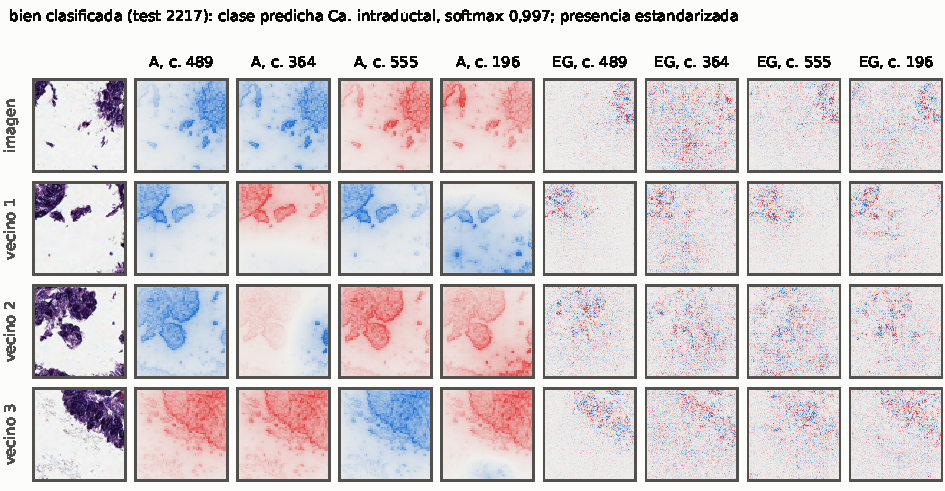
\includegraphics[width=\textwidth]{img/cap12/explicacion_id_aceptada.pdf}
  \caption{Explicación de ConvNeXt-S para una imagen ID de test bien clasificada y aceptada por \stoodx en el espacio M (\clase{Carcinoma\_intraductal}, percentil 33,7 del test ID). Filas: la imagen y sus 3 vecinos de entrenamiento según \stoodx{}. Columnas: los mapas condicionados a los 4 canales más presentes (presencia estandarizada), con la variante A de LRP y con EG condicionado. Rojo, relevancia positiva; azul, negativa; escala simétrica en el percentil 99,5 de cada mapa.}
  \label{fig:xai-id-aceptada}
\end{figure}

\begin{figure}[tbp]
  \centering
  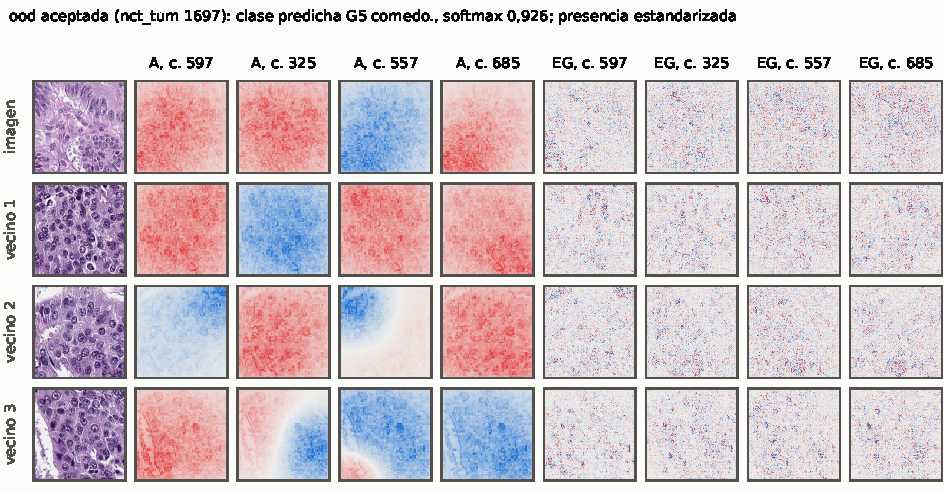
\includegraphics[width=\textwidth]{img/cap12/explicacion_ood_aceptada.pdf}
  \caption{Explicación de ConvNeXt-S para una imagen OOD (\nctcrc{} TUM) aceptada como ID por \stoodx en el espacio M (percentil 83,1 del test ID), predicha como \clase{Gleason\_5\_comedonecrosis} con \emph{softmax} 0,926. Mismo formato que la \cref{fig:xai-id-aceptada}.}
  \label{fig:xai-ood-aceptada}
\end{figure}

\section{El canal 102}\label{sec:xai-canal102}

En las primeras explicaciones, la característica más presente según la suma de valores absolutos, el criterio de la implementación pública de \stoodx (\cref{sec:stoodx-configuracion}), era siempre el canal 102 de ConvNeXt-S: aparecía entre las cuatro más presentes en los 14 casos analizados entonces y en los 16 casos de la \cref{sec:xai-casos}. Con G$\times$E, además, está entre los cuatro conceptos principales de 12 de las 14 clases en el atlas RelMax.

La \cref{fig:xai-canal102} muestra que se trata de un canal de valor grande y casi constante, no de un concepto de clase. Su media es la más baja de los 768 canales ($-9{,}90$, frente a una mediana de las medias de $-0{,}01$), es negativo en todas las imágenes de entrenamiento y es el primero tanto por media del valor absoluto como por varianza. En cambio, separa las clases como un canal cualquiera: su media por clase va de $-11{,}3$ (\clase{Gleason\_5\_no\_glandular}) a $-8{,}0$ (\clase{Gleason\_4\_glomeruloide}), su fracción de varianza entre clases, $\eta^2 = 0{,}378$, ocupa el puesto 374 de 768, en la mediana de los canales, y no está entre los 10 canales de mayor media de ninguna clase. Al estandarizar la presencia, el canal 102 desaparece de las cuatro características más presentes en los 14 casos, y en 12 de ellos cambian las cuatro.

Por tanto, la presencia medida por la suma de valores absolutos elige el canal 102 por su magnitud y no por la información que aporta sobre la clase. Es un sesgo del criterio de selección, no del modelo: un canal así llena las explicaciones sin decir nada sobre la imagen. Por ese motivo, en este capítulo las características se eligen con la presencia estandarizada.

\begin{figure}[tbp]
  \centering
  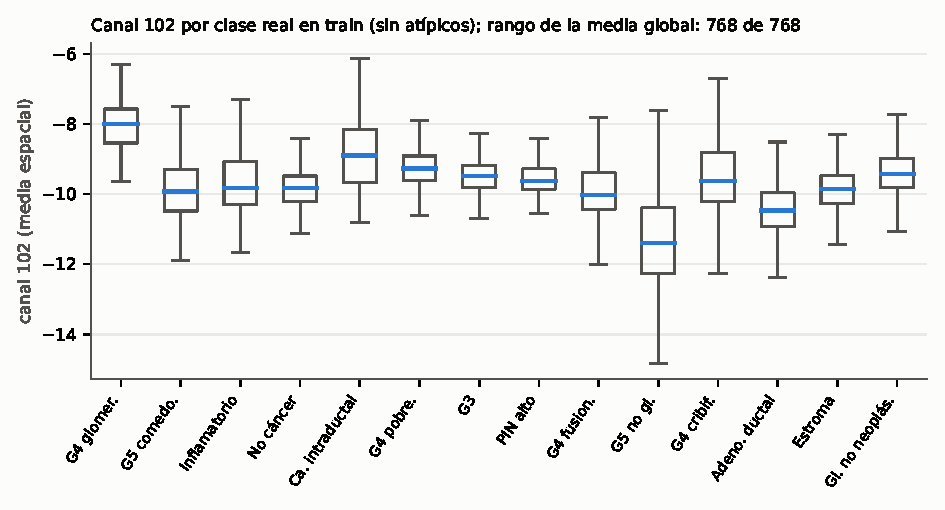
\includegraphics[width=0.8\textwidth]{img/cap12/canal102_cajas.pdf}
  \caption{Valor del canal 102 de ConvNeXt-S (media espacial de la salida del último bloque) por clase real en el conjunto de entrenamiento, sin atípicos. Su media global es la más negativa de los 768 canales y la mayor en valor absoluto.}
  \label{fig:xai-canal102}
\end{figure}

\section{Ablación de conceptos}\label{sec:xai-ablacion}

Para comprobar si los canales que cada método señala como relevantes pesan de verdad en la predicción, se sustituyen los $k$ más relevantes por su media en el entrenamiento o por cero y se mide la caída de la salida de la clase $f_c$, en las mismas 112 imágenes de test que la fidelidad.

\begin{figure}[tbp]
  \centering
  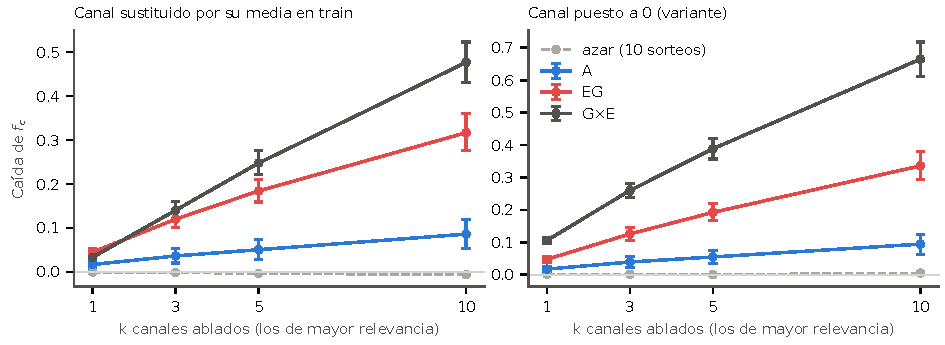
\includegraphics[width=\textwidth]{img/cap12/ablacion_conceptos.pdf}
  \caption{Caída de la salida de la clase $f_c$ de ConvNeXt-S al sustituir los $k$ canales más relevantes según la variante A de LRP, EG condicionado y Gradiente $\times$ Entrada (G$\times$E), por su media en el entrenamiento (izquierda) o por cero (derecha), frente a $k$ canales elegidos al azar. Más alto: los canales elegidos pesan más en la predicción.}
  \label{fig:xai-ablacion}
\end{figure}

% Generado por scripts/generar_tablas.py a partir de results_crp/fase10_eg/tabla/t3_ablacion.csv. No editar a mano.
\begin{table}
\centering
\scriptsize
\setlength{\tabcolsep}{3pt}
\caption{Ablación de conceptos en ConvNeXt-S (112 imágenes de test): caída media de la salida de la clase $f_c$ al sustituir los $k$ canales más relevantes de la salida del último bloque (768 canales) según cada método (por la media de train o por cero), con intervalo del 95\,\% por bootstrap.}
\label{tab:xai-ablacion}
\begin{tabular*}{\linewidth}{@{\extracolsep{\fill}}llcccc}
\toprule
Sustitución & $k$ & A & EG & G$\times$E & Azar \\
\midrule
media de train & 1 & 0{,}017 [0{,}008; 0{,}026] & 0{,}045 [0{,}036; 0{,}054] & 0{,}033 [0{,}021; 0{,}046] & $-$0{,}001 \\
 & 3 & 0{,}036 [0{,}020; 0{,}053] & 0{,}120 [0{,}101; 0{,}140] & 0{,}140 [0{,}122; 0{,}159] & $-$0{,}001 \\
 & 5 & 0{,}051 [0{,}029; 0{,}073] & 0{,}184 [0{,}159; 0{,}210] & 0{,}248 [0{,}221; 0{,}276] & $-$0{,}004 \\
 & 10 & 0{,}086 [0{,}053; 0{,}119] & 0{,}317 [0{,}275; 0{,}360] & 0{,}477 [0{,}432; 0{,}523] & $-$0{,}006 \\
\midrule
cero & 1 & 0{,}017 [0{,}009; 0{,}026] & 0{,}048 [0{,}039; 0{,}057] & 0{,}106 [0{,}097; 0{,}115] & 0{,}001 \\
 & 3 & 0{,}039 [0{,}024; 0{,}055] & 0{,}126 [0{,}107; 0{,}146] & 0{,}260 [0{,}239; 0{,}282] & 0{,}002 \\
 & 5 & 0{,}055 [0{,}035; 0{,}076] & 0{,}192 [0{,}167; 0{,}219] & 0{,}389 [0{,}357; 0{,}421] & 0{,}001 \\
 & 10 & 0{,}095 [0{,}063; 0{,}125] & 0{,}336 [0{,}293; 0{,}381] & 0{,}665 [0{,}613; 0{,}718] & 0{,}006 \\
\bottomrule
\end{tabular*}

\smallskip
\parbox{\linewidth}{\scriptsize Más alto: los canales elegidos pesan más en la predicción. Azar: media de 10 sorteos de $k$ canales.}
\end{table}


Los tres métodos eligen canales que pesan más que los elegidos al azar, cuya caída es prácticamente nula (\cref{tab:xai-ablacion}). La variante A es, con diferencia, la que menos acierta: al sustituir sus 10 canales más relevantes por la media de entrenamiento, $f_c$ cae 0,086, frente a 0,317 con EG y 0,477 con G$\times$E. La diferencia entre EG y la variante A es positiva, con el intervalo por encima de cero, para todos los $k$ y las dos sustituciones. G$\times$E supera a EG en casi todos los casos, salvo con un solo canal sustituido por la media, donde EG es ligeramente mejor (+0,012 [0,001; 0,024]). La ventaja de G$\times$E es mayor al sustituir por cero, lo que era de esperar: con la sustitución por cero, su relevancia por canal coincide casi exactamente con la caída que produce ese canal (correlación de Pearson 0,999), mientras que con la media de entrenamiento la correlación baja a 0,918. Los métodos de gradiente, en resumen, identifican mejor los canales de los que depende la predicción que la variante A de LRP.

\section{Atlas RelMax}\label{sec:xai-atlas}

Para describir qué representa cada concepto se ha construido un atlas RelMax (\cref{sec:crp-relmax}): para cada clase se eligen sus cuatro canales más relevantes en el test y, para cada canal, las ocho imágenes de entrenamiento en las que tiene mayor relevancia normalizada. Por coste, las referencias se buscan en una muestra estratificada del entrenamiento (el 5\,\% de cada clase, con un mínimo de 50 imágenes; \num{4654} en total). La \cref{fig:xai-atlas-estroma} muestra el atlas de la clase \clase{Estroma}.

\begin{figure}[tbp]
  \centering
  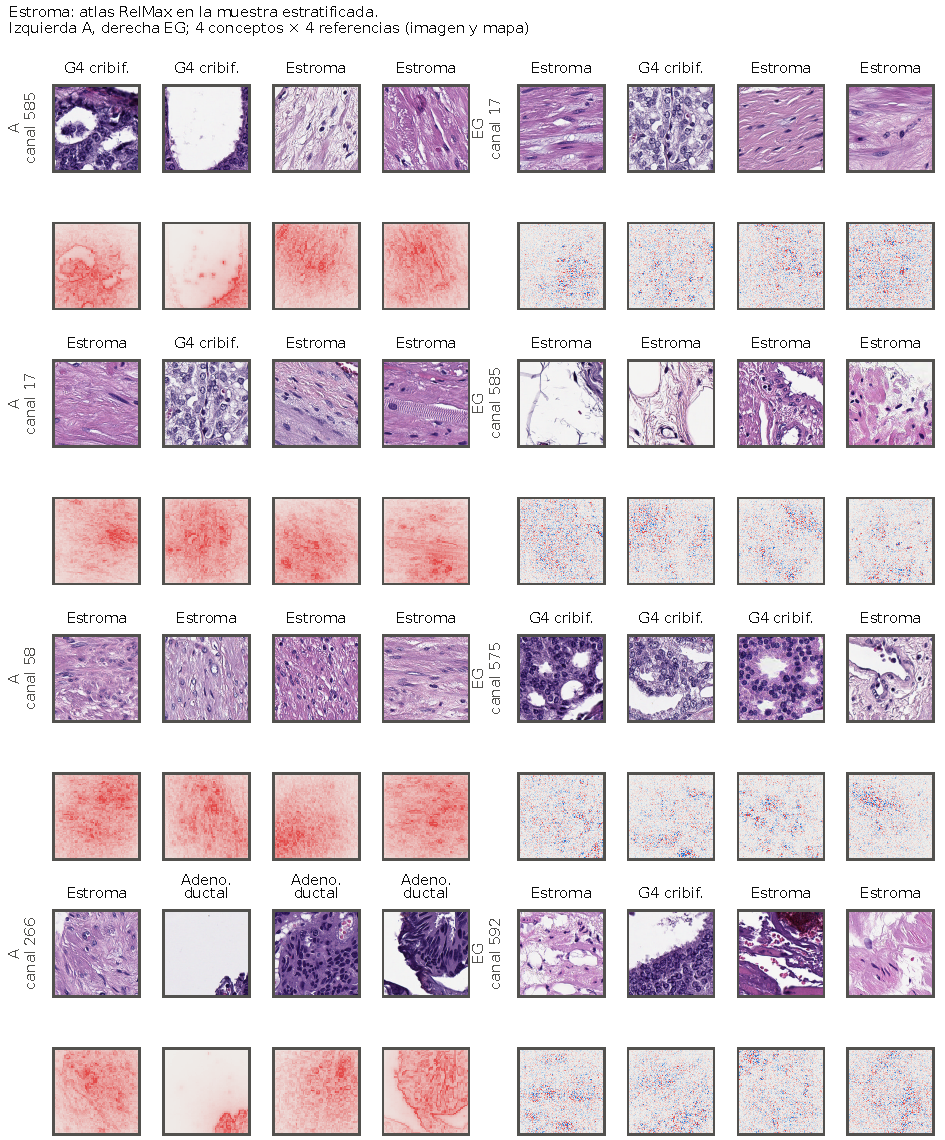
\includegraphics[width=\textwidth]{img/cap12/atlas_relmax_estroma.pdf}
  \caption{Atlas RelMax de la clase \clase{Estroma} en ConvNeXt-S, sobre una muestra estratificada del entrenamiento: los 4 conceptos (canales) de la clase con la variante A de LRP (izquierda) y con EG condicionado (derecha) y, para cada concepto, 4 de sus 8 referencias, con la imagen y su mapa condicionado. Sobre cada imagen, su clase real.}
  \label{fig:xai-atlas-estroma}
\end{figure}

% Generado por scripts/generar_tablas.py a partir de results_crp/fase10_eg/{paso4/muestra/resultados,tabla,comprobaciones_finales}. No editar a mano.
\begin{table}
\centering
\small
\caption{Atlas RelMax de ConvNeXt-S (4 conceptos por clase y 8 referencias por concepto).}
\label{tab:xai-atlas}
\begin{tabular*}{\linewidth}{@{\extracolsep{\fill}}lcc}
\toprule
Atlas & Clase del concepto & Clase mayoritaria \\
\midrule
EG, muestra, semilla 0 & 0{,}625 & 0{,}750 \\
EG, muestra, semilla 1 & 0{,}750 & 0{,}750 \\
A, muestra & 0{,}375 & 0{,}625 \\
A, train completo & 0{,}500 & 0{,}625 \\
G$\times$E, train completo & 0{,}625 & 1{,}000 \\
\midrule
\multicolumn{3}{@{}l}{\textit{Estabilidad de EG entre semillas (43 canales concepto)}} \\
Referencias comunes del top-8, mediana [mín.; máx.] & \multicolumn{2}{c}{3 [0; 6]} \\
Conceptos con solape bajo ($\le 4$ de 8) & \multicolumn{2}{c}{42 de 43} \\
Spearman en las 50 candidatas, mediana & \multicolumn{2}{c}{0{,}295} \\
\midrule
\multicolumn{3}{@{}l}{\textit{Solapes}} \\
Conceptos comunes EG y A (de 56) & \multicolumn{2}{c}{26} \\
Referencias comunes EG y A (de 8, media) & \multicolumn{2}{c}{0{,}59} \\
Referencias comunes A muestra y A train completo (de 8, media) & \multicolumn{2}{c}{0{,}54} \\
\bottomrule
\end{tabular*}

\smallskip
\parbox{\linewidth}{\scriptsize Pureza: mediana de la fracción de las 8 referencias que son de la clase del concepto o de su clase mayoritaria (más alto, referencias más homogéneas). Muestra: muestra estratificada del train (5\,\% por clase, mínimo 50; 4.654 imágenes). Con la semilla 1, el top-8 se elige entre las 50 candidatas de la semilla 0. Los solapes de referencias se dan en los canales concepto.}
\end{table}


Con la variante A, varias referencias de \clase{Estroma} no son estroma: el canal 585 incluye imágenes de \clase{Gleason\_4\_cribiformes} con una luz glandular grande, y el canal 266, imágenes de \clase{Adenocarcinoma\_ductal}, una de ellas casi enteramente de fondo blanco, con la relevancia en el borde del tejido. Con EG, las referencias son más homogéneas (por ejemplo, las cuatro mostradas del canal 585 son de \clase{Estroma}), pero sus mapas vuelven a ser ruido de píxel sin estructura apreciable. La \cref{tab:xai-atlas} lo cuantifica: la mediana de la fracción de referencias de la clase del concepto es 0,625 con EG y 0,375 con la variante A en la misma muestra, y la diferencia de medias es positiva con intervalo por encima de cero con las dos semillas de EG. Sin embargo, las referencias concretas de EG son poco estables: entre dos semillas comparten una mediana de 3 de las 8, y 42 de los 43 canales concepto tienen un solape de 4 o menos. Los dos métodos coinciden en 26 de los 56 conceptos, pero apenas en sus referencias (0,59 de 8 de media).

\section{Discusión}\label{sec:xai-discusion}

Las explicaciones obtenidas no permiten identificar con seguridad en qué se apoya el clasificador. La variante A de LRP conserva la relevancia, pero sus mapas condicionados se parecen entre conceptos, apenas cambian al aleatorizar el modelo, eligen canales que pesan poco en la predicción y llevan al atlas referencias de otras clases. Es coherente con el olvido de la relevancia inicial que predice el análisis de la regla $z^{+}$ como cadena de Markov (\cref{sec:lrp-markov}). EG es más fiel y sus conceptos son más puros, pero sus mapas condicionados, con 128 referencias, están dominados por el ruido de muestreo, y sus referencias cambian con la semilla.

Aun así, el análisis aporta dos resultados útiles. El primero es que el criterio de presencia por suma de valores absolutos está sesgado hacia los canales de gran magnitud, como el 102, y conviene estandarizarlo antes de usarlo para explicar o para seleccionar características. El segundo es que el borde entre el tejido y el fondo blanco aparece de forma repetida en los mapas de la variante A y en las referencias de algunos conceptos. Esto no basta para afirmar que el modelo use el fondo como atajo, pero encaja con lo observado en PANDA, que contiene mucho más fondo blanco que el conjunto ID (\cref{sec:ood-panda}), y es una pista que habría que contrastar eliminando o enmascarando esos conceptos, como en el caso de la marca de agua de Achtibat et al.~\cite{achtibat2023}. Esa intervención, la eliminación de los conceptos sesgados y su efecto sobre la exactitud y la detección OOD, queda como trabajo futuro (\cref{sec:trabajo-futuro}).

\endinput
